\chapter{Design of uROS}
\section{RCLC}
\subsection{RCLC-Executor}
Here we introduce the rclc Executor, which is a ROS 2 Executor implemented based on and for the rcl API, for applications written in the C language. Often embedded applications require real-time to guarantee end-to-end latencies and need deterministic runtime behavior to correctly replay test data. However, this is difficult with the default ROS 2 Executor because of its complex semantics, as discussed in the previous section.

First, we will analyse the requirements for real-time embedded applications and, secondly, derive simple features for an Executor to enable deterministic and real-time behavior. Then we will present the API of the RCLC-Executor and provide example usages of the RCLC-Executor to address these requirements.

\subsubsection{Requirement Analysis}
\todo{Real-time embedded application use-case and LET\footnote{https://github.com/ros2/rclc/tree/master/rclc}}

The described embedded use case relies on the following concepts:
\begin{itemize}
    \item [(1)] periodic execution of processes
    \item [(2)] assignment of fixed priorities to processes
    \item [(3)] preemptive scheduling of processes
    \item [(4)] co-operative scheduling of tasks within a process (sequential execution)
    \item [(5)] data synchronization with LET-semantics
\end{itemize}

While \underline{periodic activation} is possible in ROS 2 by using timers, \underline{preemptive scheduling} is supported by the operating system and \underline{assigning priorities} on the granularity of threads/processes that correspond to the ROS nodes; it is not possible to \underline{sequentially execute callbacks}, which have no data-dependency. Furthermore data is read from the DDS queue just before the callback is executed and data is written sometime during the time the application is executed. While the \api{spin\_period} function of the rclcpp-Executor allows to check for data at a fixed period and executing those callbacks for which data is available, however, with this spin-function does not execute all callbacks irrespective whether data is available or not. So \api{spin\_period} is not helpful to periodically execute a number of callbacks (aka tasks within a process). So we need a mechanism that triggers the execution of multiple callbacks (aka tasks) based on a timer. Data transmission is achieved via DDS which does not allow to implement a LET-semantics. To summarize, we derive the following requirements:
\begin{itemize}
    \item [(1)] trigger the execution of multiple callbacks
    \item [(2)] sequential processing of callbacks
    \item [(3)] data synchronization with LET semantics
\end{itemize}

\subsubsection{RCLC-Executor Features}
Based on the real-time embedded use cases as well as the software architecture patterns in mobile robotics, RCLC-Executor are proposed with the following main features:

\textbf{User-defined sequential execution of callbacks:} At configuration, the user defines the order of handles and whether the handle shall be called only when new data is available (ON\_NEW\_DATA) or whether the callback shall always be called (ALWAYS). At runtime, all handles are processed in the user-defined order: if the configuration of handle is ON\_NEW\_DATA, then the corresponding callback is only called if new data is available; if the configuration of the handle is ALWAYS, then the corresponding callback is always executed. In case, no data is available from DDS, then the callback is called with no data (e.g. NULL pointer).

\textbf{Trigger condition to activate processing:} Given a set of handles, a trigger condition based on the input data of these handles shall decide when the processing is started. Available options include: ALL operation, fires when input data is available for all handles; ANY operation, fires when input data is available for at least one handle; ONE, fires when input data for a user-specified handle is available; User-defined function, user can implement more sophisticated logic.

\textbf{LET-Semantics:} 
\begin{itemize}
    \item Assumption: time-triggered system, the executor is activated periodically
    \item When the trigger fires, reads all input data and makes a local copy
    \item Processes all callbacks in sequential order
    \item Write output data at the end of the executor's period (Note: this is not implemented yet)
\end{itemize}

Additionally the rclcpp Executor semantics (RCLCPP) is implemented and chosen as the default configuration:
\begin{itemize}
    \item waiting for new data for all handles (rcl\_wait)
    \item using trigger condition ANY
    \item if trigger fires, start processing handles in pre-defined sequential order
    \item request from DDS-queue the new data just before the handle is executed (rcl\_take)
\end{itemize}




\section{RCL}

\section{RMW}

\section{XRCE-DDS}
\textbf{eProsima Micro XRCE-DDS} is an open-source wire protocol that implements the OMG DDS for e\textbf{X}tremely \textbf{R}esource \textbf{C}onstrained \textbf{E}nvironment standard (DDS-XRCE). The aim of the DDS-XRCE protocol is to provide access to the DDS Global-Data-Space from resource-constrained devices. This is achieved thanks to a client-server architecture, where low resource devices (called XRCE Clients), are connected to a server (called XRCE Agent), which acts on behalf of its clients in the DDS Global-Data-Space.
\begin{figure}[htb!]
    \centering
    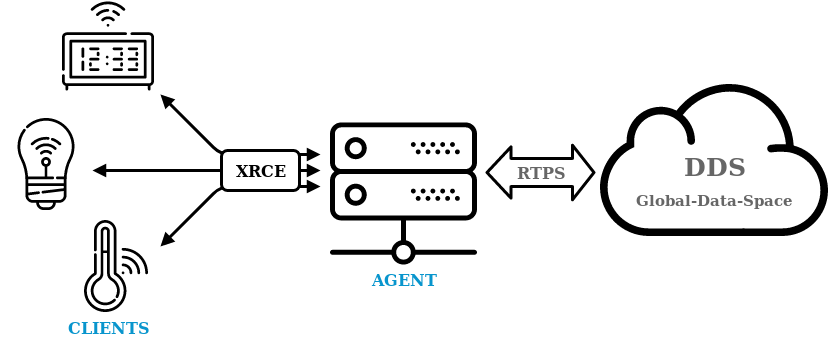
\includegraphics[width=0.95\linewidth]{Img/uxrce_scope.png}
    \caption{structure}\label{f:uxrce}
    \vspace{-0.1in}
\end{figure}

Micro XRCE-DDS is composed by two main elements:
\begin{itemize}
    \item \textbf{Micro XRCE-DDS Agent}: a C++11 out-of-the-box application which implements the XRCE Agent functionality
    \item \textbf{Micro XRCE-DDS Client}: a C99 library which implements the XRCE Client side functionality
\end{itemize}

In addition, Micro XRCE-DDS uses other two components:
\begin{itemize}
    \item \textbf{Micro CDR}: a \underline{de/serialization engine} used in the Client library
    \item \textbf{Micro XRCE-DDS Gen}: a code generator tool used for generating Micro CDR de/serialization functions and Client apps examples from IDL sources.
\end{itemize}

\subsection{Main Features}
\textbf{1. Low Resource Consumption}: As it was mentioned above, Micro XRCE-DDS is focused on microcontroller applications. Therefore, the design and implementation of this middleware have been carried out taking into account the memory constraints of this kind of devices. A proof of this is the fact that the XRCE Client is completely \underline{dynamic memory free}. From the point of view of the memory footprint, the latest version of this library has a memory consumption of less than 75 KB of Flash memory and around 3 KB of RAM for a complete publisher and subscriber application handling messages sizes on the order of 512 B. For more detailed information on the memory consumption as a function of message size, entity number and internal memory management of the middleware library, please refer to the \href{https://micro.ros.org/docs/concepts/middleware/memo_prof/}{Micro XRCE-DDS memory profiling section}. Moreover, this library is highly configurable thanks to a profile concept that enables to choose, add or remove some features in configuration time. That allows customizing the XRCE Client library size, if there are features that are not used. There are several definitions for configuring and building the Client library at compile-time. These definitions allow to create a version of the library according to the application requirements, and can be modified in the client.config file. For incorporating the desired configuration, it is necessary to run the cmake command every time the definitions change.

\textbf{2. Multi-Transport Support}: As part of the profiles discussed in the previous section, the user can choose between several transport layers to communicate the Clients with the Agent. Indeed, in contrast to other IoT middleware such as MQTT and CoaP, which work over only a particular transport layer, XRCE supports multiple transport protocols natively. In particular, the latest version of Micro XRCE-DDS support: UDP, TCP and a custom Serial transport protocol. Apart from this, Micro XRCE-DDS has a transport interface for both Agent and Client which allows to implement custom transports in a straightforward manner. This makes the port of Micro XRCE-DDS to different platforms and the addition of new transports a seamless task that any user can undertake.

\textbf{3. Multi-Platform Support}: The XRCE Client supports FreeRTOS, Zephyr and NuttX as embedded RTOS. Moreover, it also runs on Windows and Linux. On the other hand, the XRCE Agent supports Windows and Linux.

\textbf{4. QoS support}: The XRCE Client library allows the user to use two different approaches for creating DDS entities in the XRCE Agent: By XML (the default option), By reference. When using the default option, users are enabled to create entities either in Reliable or Best-Effort mode, with the XML files written and stored on the Client side. But these QoS configurations may not fit some users’ requirements. For these cases, Micro XRCE-DDS allows to create entities directly on the Agent, where the user can write custom XML QoS as in DDS. Each entity available on the Agent will be associated to a label, so that the Clients can to create the entities they need for the communication by just referring to these labels. Additionally, using references will also reduce the memory consumption of the Client inside the MCU. This is because the reference approach allows avoiding to build the parts of the code where XMLs are stored.

\subsection{Micro XRCE-DDS Client}
The Micro XRCE-DDS Clients\footnote{Github: https://github.com/eProsima/Micro-XRCE-DDS-Client} are lightweight entities meant to be compiled on eXtremely Resource Constrained Environments.
\begin{figure}[htb!]
    \centering
    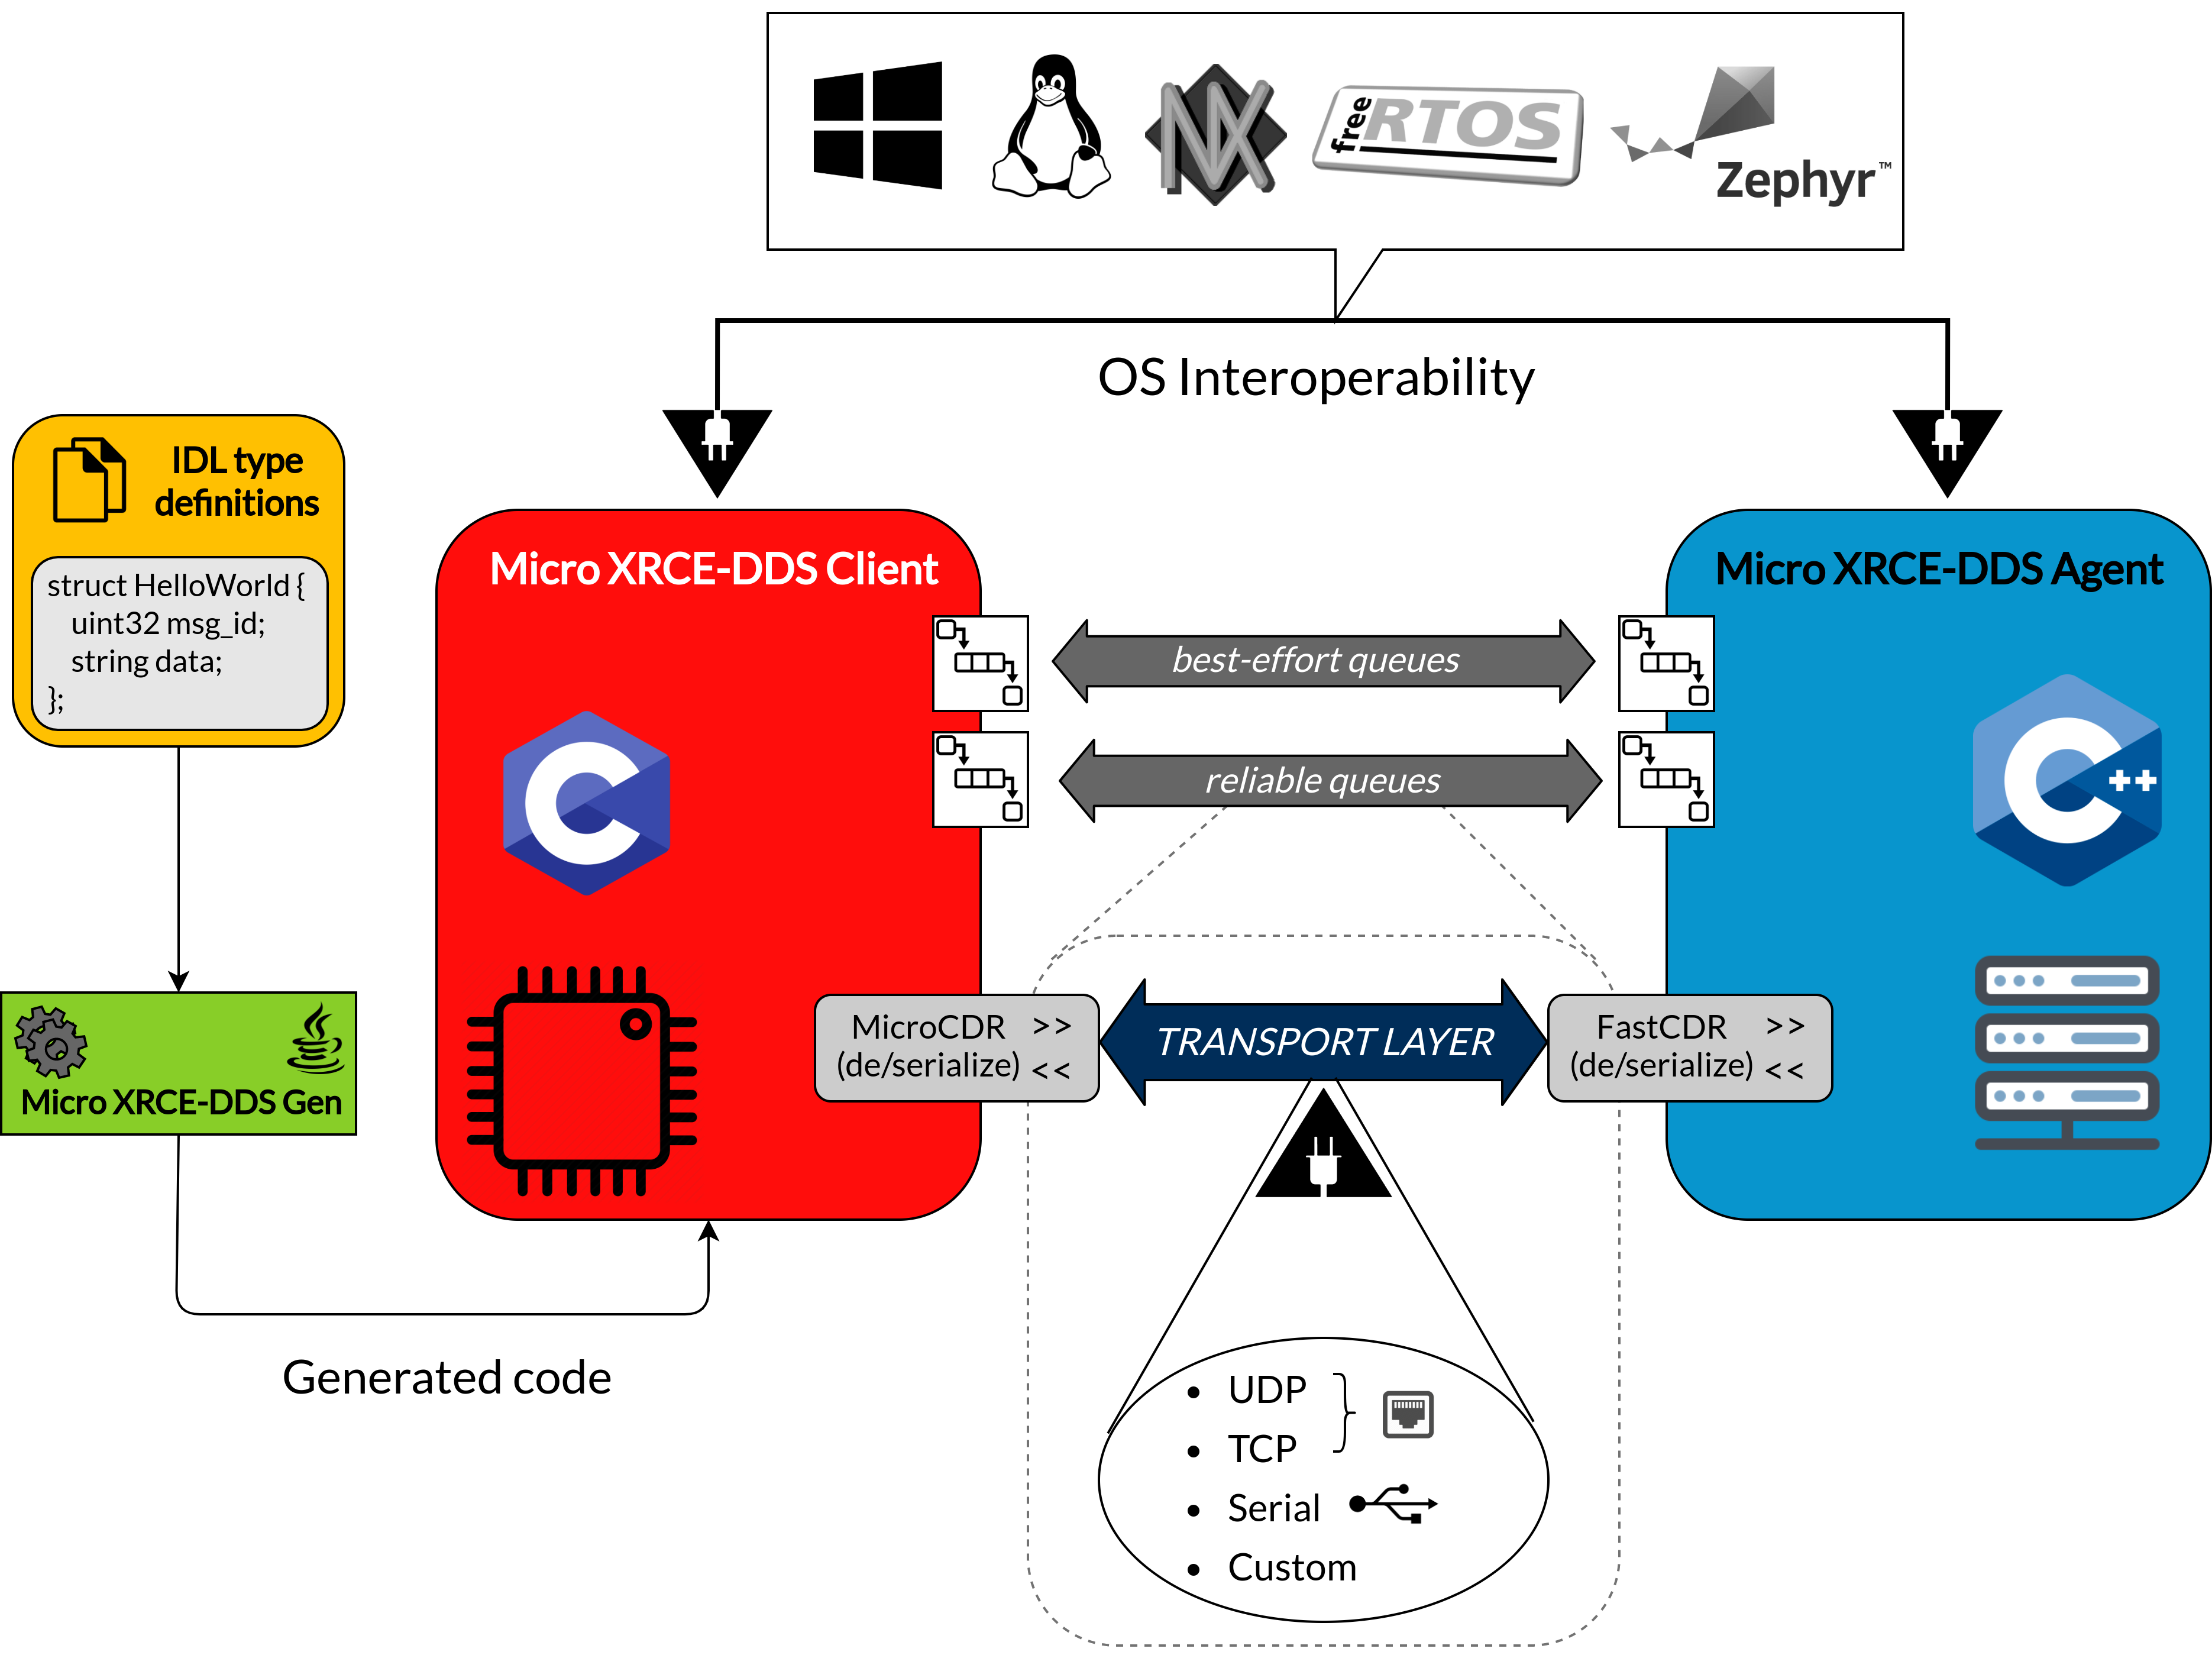
\includegraphics[width=0.95\linewidth]{Img/General.png}
    \caption{structure}\label{f:general}
    \vspace{-0.1in}
\end{figure}

The Micro XRCE-DDS Clients request operations to the Agent to publish and/or subscribe to topics in the DDS global dataspace. Remote procedure calls, as defined by the DDS-RPC standard, are also supported, allowing Clients to communicate in the DDS dataspace according to a request/reply paradigm. The Agents process these requests and send back a response with the operation status result and with the requested data, in the case of subscribe/reply operations. The communication in the DDS world is mediated by a dedicated ProxyClient in charge of creating the DDS Entities requested by the Clients, such as Participants, Topics, Publishers, and Subscribers, which can interact with the DDS Global dataspace.
\begin{figure}[htb!]
    \centering
    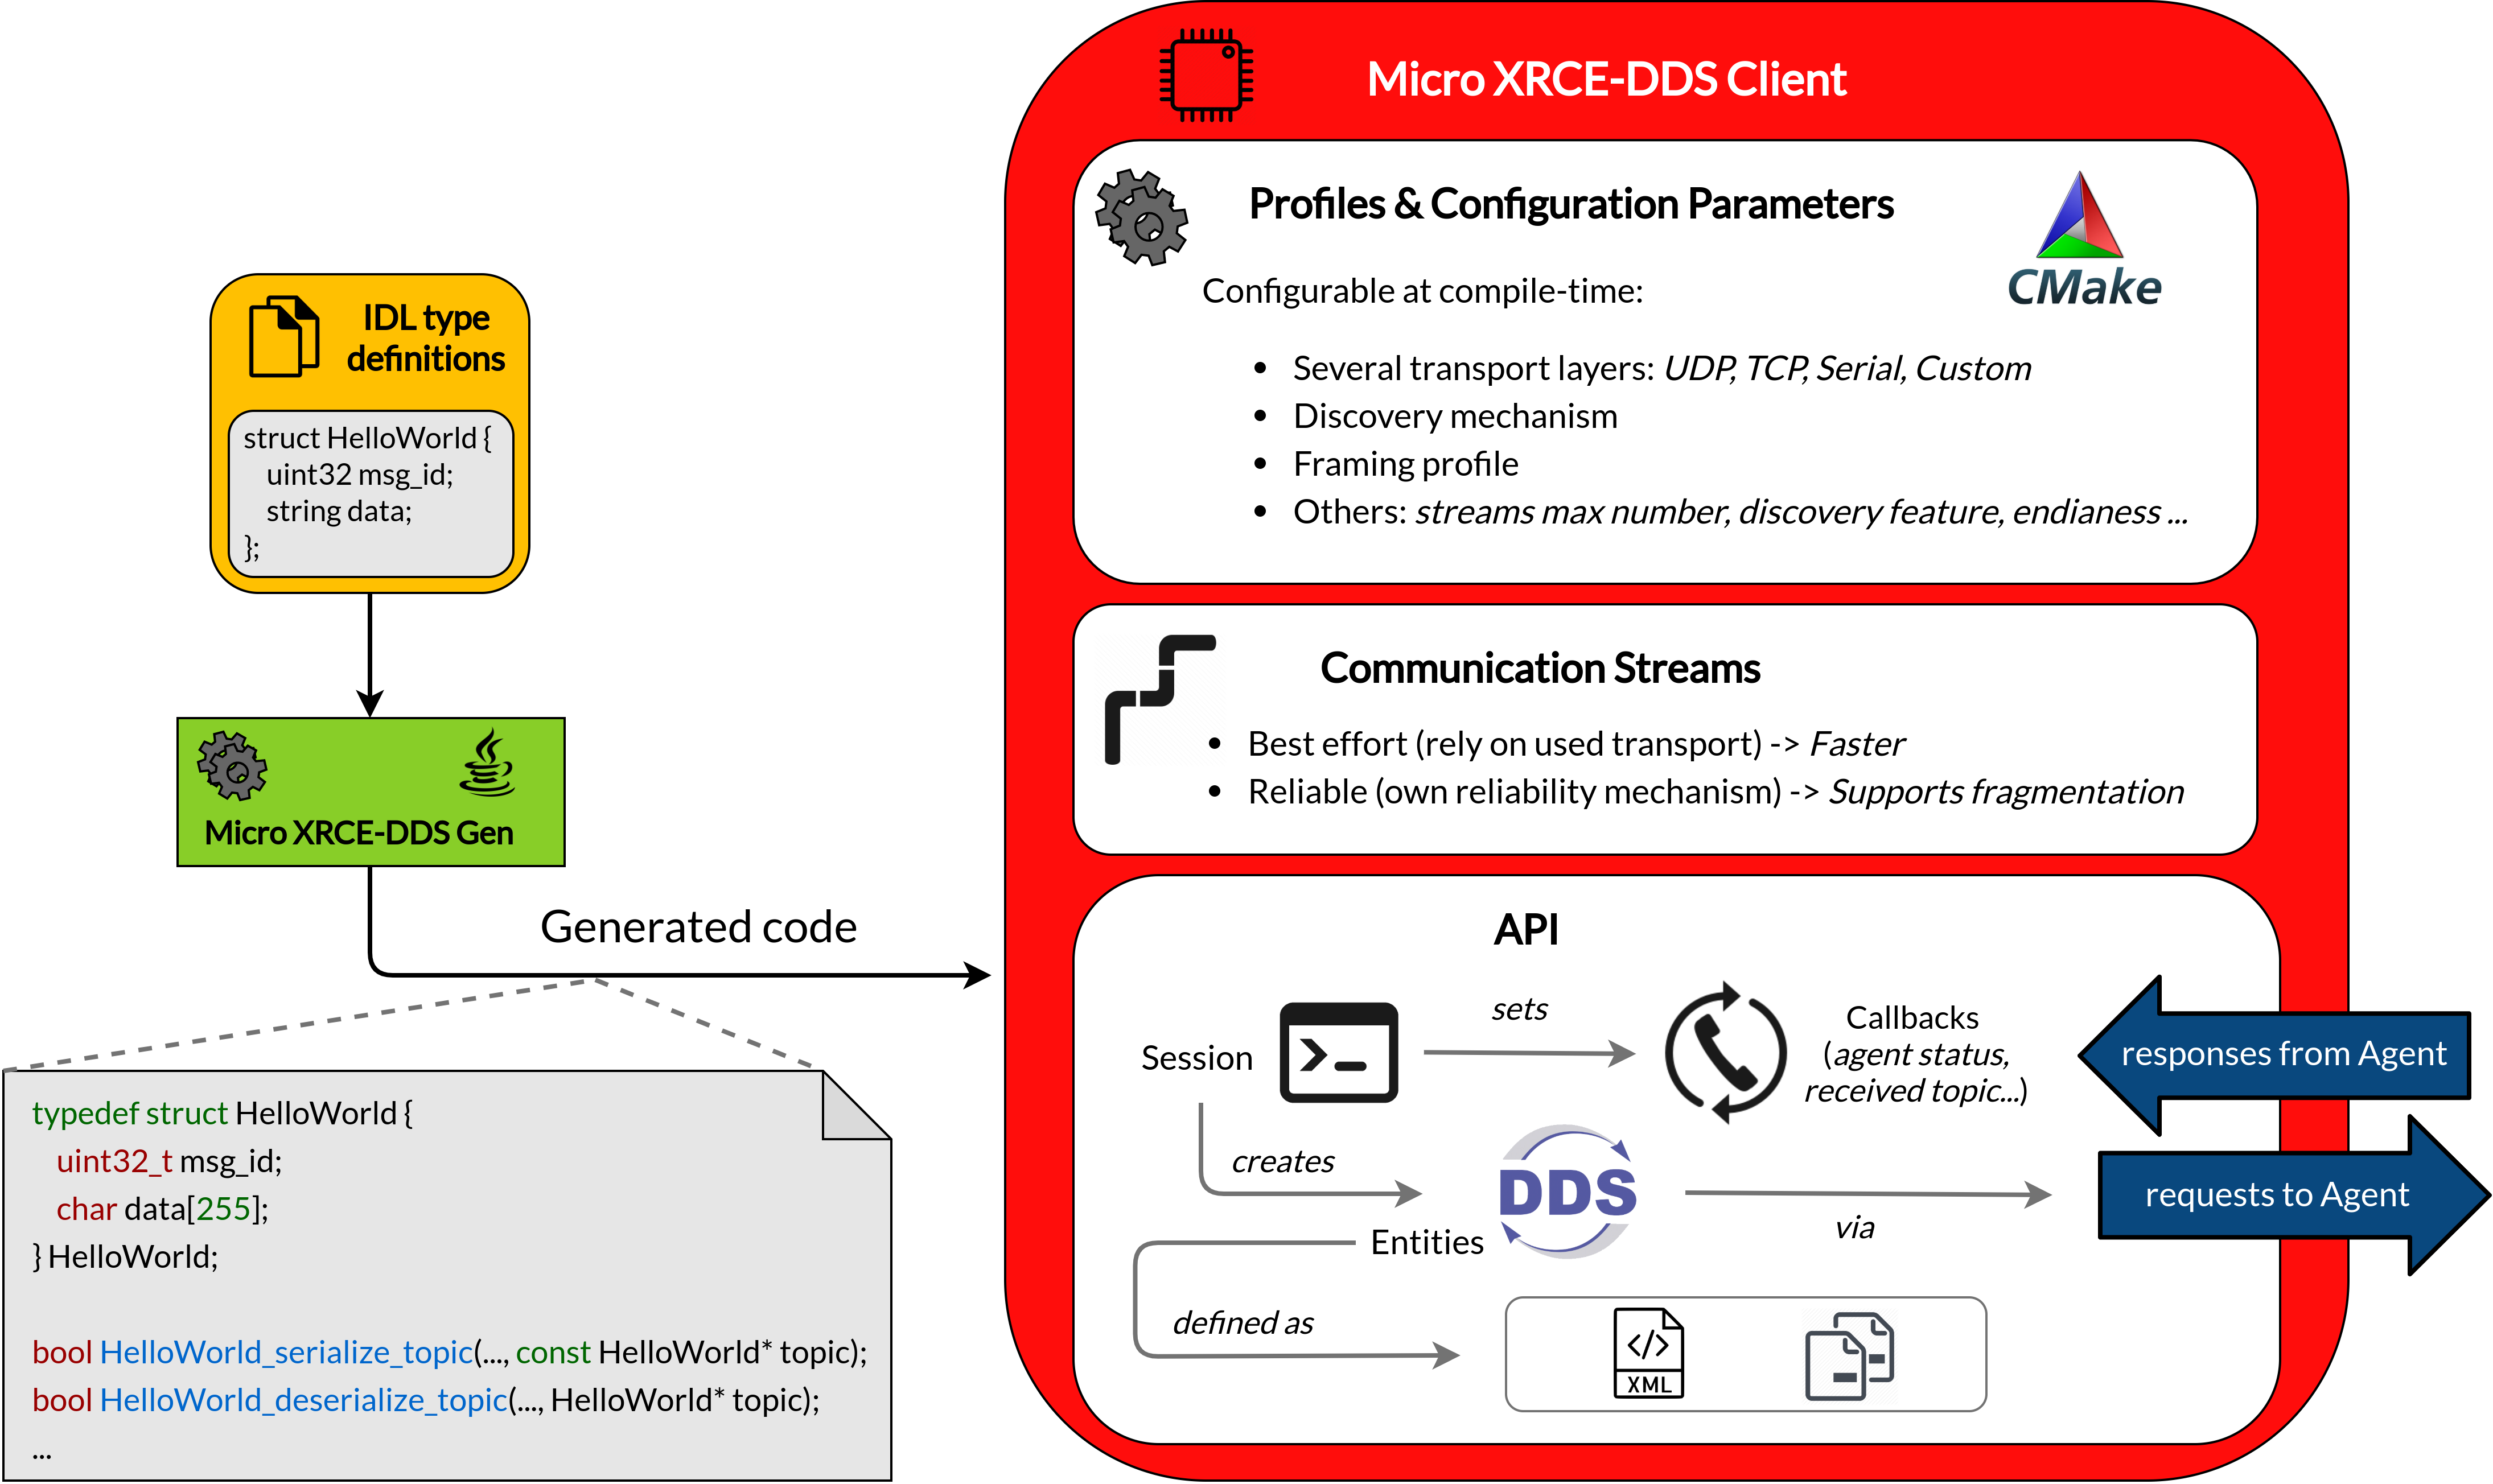
\includegraphics[width=0.95\linewidth]{Img/Client.png}
    \caption{client}\label{f:client}
    \vspace{-0.1in}
\end{figure}
eProsima Micro XRCE-DDS provides the user with a C API to create Micro XRCE-DDS Clients applications. The library can be configured at compile-time via a set of CMake flags allowing to enable or disable some profiles before compilation, and to manipulate several parameters controlling some of the library's functionalities, which in turn allow tuning the library size.

The communication between a Micro XRCE-DDS Client and a Micro XRCE-DDS Agent is achieved by means of several kinds of built-in transports: UDPv4, UDPv6, TCPv4, TCPv6 and Serial communication. In addition, there is the possibility for the user to generate its own Custom transport.

\subsection{Micro XRCE-DDS Agent} 
The Micro XRCE-DDS Agent\footnote{Github: https://github.com/eProsima/Micro-XRCE-DDS-Agent} is a broker which bridges the Clients with the DDS world.
\section{USED POSIX API}